\begin{figure}[H]
	\centering
	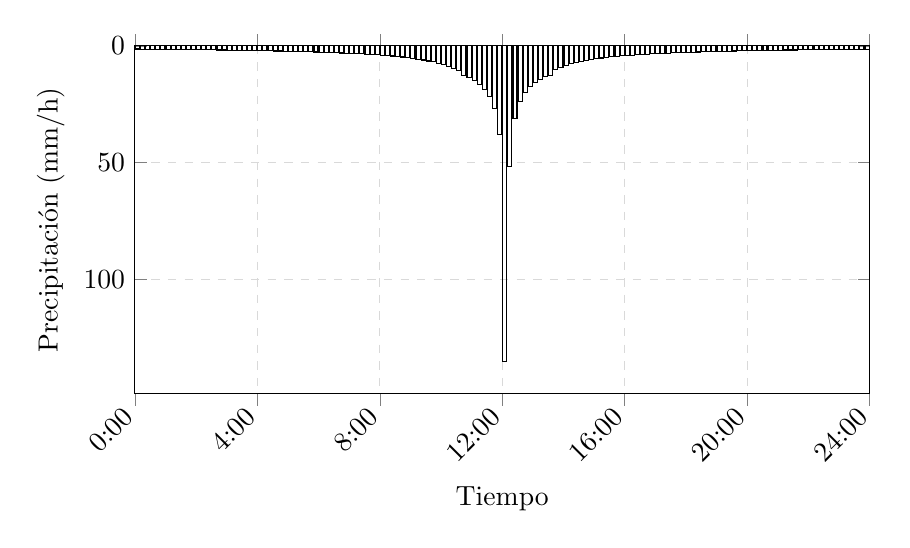
\begin{tikzpicture}
		\begin{axis}[
			width=0.9\textwidth,
			height=6cm,
			xlabel={Tiempo},
			ylabel={Precipitación (mm/h)},
			y dir=reverse,
			ymin=0,
			ymax=149,
			xmin=0,
			xmax=1440,
			ybar,
			bar width=8,
			xtick={0, 240, 480, 720, 960, 1200, 1440},
			xticklabels={0:00, 4:00, 8:00, 12:00, 16:00, 20:00, 24:00},
			xticklabel style={rotate=45, anchor=east},
			grid=major,
			grid style={dashed, gray!30},
			]
			\addplot [
			draw=black,
			fill=none
			]
			coordinates {
				(5, 1.38) (15, 1.44) (25, 1.44) (35, 1.50) (45, 1.50)
				(55, 1.50) (65, 1.56) (75, 1.56) (85, 1.56) (95, 1.62)
				(105, 1.62) (115, 1.68) (125, 1.68) (135, 1.68) (145, 1.74)
				(155, 1.74) (165, 1.80) (175, 1.80) (185, 1.86) (195, 1.86)
				(205, 1.92) (215, 1.98) (225, 1.98) (235, 2.04) (245, 2.10)
				(255, 2.10) (265, 2.16) (275, 2.22) (285, 2.22) (295, 2.28)
				(305, 2.34) (315, 2.40) (325, 2.46) (335, 2.52) (345, 2.58)
				(355, 2.64) (365, 2.70) (375, 2.82) (385, 2.88) (395, 2.94)
				(405, 3.06) (415, 3.12) (425, 3.30) (435, 3.36) (445, 3.48)
				(455, 3.60) (465, 3.72) (475, 3.90) (485, 4.02) (495, 4.26)
				(505, 4.38) (515, 4.68) (525, 4.80) (535, 5.10) (545, 5.40)
				(555, 5.70) (565, 6.06) (575, 6.48) (585, 6.90) (595, 7.50)
				(605, 8.10) (615, 8.82) (625, 9.66) (635, 10.74) (645, 12.78)
				(655, 13.68) (665, 14.88) (675, 16.50) (685, 18.60) (695, 21.72)
				(705, 26.82) (715, 37.86) (725, 135.36) (735, 51.84) (745, 31.02)
				(755, 23.88) (765, 19.98) (775, 17.46) (785, 15.66) (795, 14.34)
				(805, 13.20) (815, 12.66) (825, 10.20) (835, 9.24) (845, 8.46)
				(855, 7.74) (865, 7.20) (875, 6.72) (885, 6.30) (895, 5.88)
				(905, 5.58) (915, 5.22) (925, 5.04) (935, 4.74) (945, 4.50)
				(955, 4.32) (965, 4.14) (975, 3.96) (985, 3.84) (995, 3.66)
				(1005, 3.54) (1015, 3.42) (1025, 3.30) (1035, 3.18) (1045, 3.12)
				(1055, 3.00) (1065, 2.94) (1075, 2.82) (1085, 2.76) (1095, 2.70)
				(1105, 2.64) (1115, 2.52) (1125, 2.52) (1135, 2.40) (1145, 2.40)
				(1155, 2.34) (1165, 2.28) (1175, 2.22) (1185, 2.16) (1195, 2.10)
				(1205, 2.10) (1215, 2.04) (1225, 1.98) (1235, 1.98) (1245, 1.92)
				(1255, 1.92) (1265, 1.86) (1275, 1.80) (1285, 1.80) (1295, 1.80)
				(1305, 1.74) (1315, 1.74) (1325, 1.68) (1335, 1.68) (1345, 1.62)
				(1355, 1.62) (1365, 1.56) (1375, 1.56) (1385, 1.56) (1395, 1.56)
				(1405, 1.50) (1415, 1.50) (1425, 1.44) (1435, 1.44)
			};
		\end{axis}
	\end{tikzpicture}
	\caption{Hietograma - BLOCKS24 $T_r$=10 años (P=151.8 mm)}
	\label{fig:hyeto_kirpich_blocks24_Tr10}
\end{figure}
